\chapter{Implementing Internal Model Controller for first order systems}
The aim of this experiment is to implement an Internal Model Controller(IMC) for first order systems on a single board heater system. The target group is anyone who has a basic knowledge of Control Engineering.
\begin{figure}
	\centering
		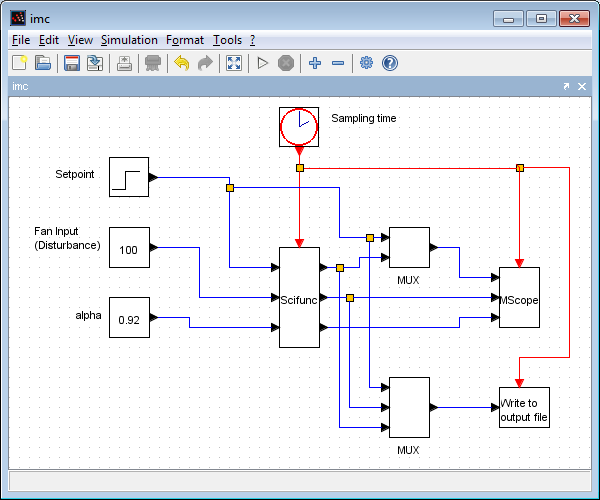
\includegraphics[width=\linewidth]{IMC/imc_xcos.png}
	\caption{Xcos interface for this experiment}
	\label{Xcos_imc}
\end{figure}
Scilab with Xcos has been used as an interface for sending and receiving data. This interface is shown in Fig.\ref{Xcos_imc}.Fan speed and Heater current are the two inputs to the system. For this experiment, the heater current is used as a control effort and the fan input could be thought of as an external disturbance.

\section{IMC Design for Single Board Heater System}
Internal Model Controller contains the explicit model of the plant as its part, hence it is named as Internal Model Controller \cite{kmm09}. 
If the open loop transfer function and controller are stable, the closed loop system can be stabilized. The IMC is generally used for stable plants.\\
\begin{figure}
\begin{center}
\begin{tikzpicture}[auto,node distance=2cm]
\node[input](input){};
\node[sum,right of=input](sum1){};
\draw[->](input)--node{$r$}(sum1);
\node[block,right of=sum1](gqz){$G_Q(z)$};
\draw[->](sum1)--node{$e$}(gqz);
\node[branch,right of=gqz, node distance=2cm](b1){};
\node[block, right of=b1](gpz){$G_p(z)$};
\draw[->](gqz)--node{$u$}(gpz);
\node[sum, right of=gpz,pin={[pinstyle] above:$\xi$},node distance=2cm](sum2){};
\draw[->](gpz)--(sum2);
\node[output, right of=sum2](output){};
\draw[->](sum2)--node{$y$}(output);
\node[branch, right of=sum2, node distance=1cm](b2){};
\node[sum, below of=b2,node distance=2cm](sum3){};
\draw[->](b2)--(sum3);
\node[block,below of=gpz](gz){$G(z)$};
\draw[->](b1)|-(gz);
\draw[->](gz)--node{$\bar{y}$\hspace{0.7cm} $-$}(sum3);
\draw[->](sum3)--(10,-3)-|node[pos=0.88]{$-$}(sum1);
\end{tikzpicture}
\end{center}
\caption{IMC feedback configuration}
\label{imcfeedback}
\end{figure}

Let the transfer function of the stable plant be denoted by $G_p (z)$ and it's model be denoted by $G(z)$.Then,
\begin{align}
y(n)=G(z)u(n)+\xi(n) 
\end{align}
where; \\
y(n)=plant output;\\
u(n)=plant input;\\
$\xi$(n)=noise.
      
Fig.\ref{imcfeedback} shows the block diagram representation of an IMC.
For noise rejection ($\xi$=0) and no plant-model mismatch($G=G_p$), $G_Q=G_p^{-1}$ i.e. for stable $G_Q$ an approximate inverse of G is required.Also, for internal stability, transfer function between any two points in the feedback loop must be stable.\cite{kmmdc09}
\begin{figure}
\begin{center}
\begin{tikzpicture}[auto,node distance=2cm]
\node[input](input){};
\node[sum,right of=input](sum1){};
\draw[->](input)--node{$r$}(sum1);
\node[sum, right of=sum1](sum2){};
\draw[->](sum1)--(sum2);
\node[block,right of=sum2](gqz){$G_Q(z)$};
\draw[->](sum2)--node{$e$}(gqz);
\node[branch,right of=gqz, node distance=2cm](b1){};
\node[block, right of=b1](gpz){$G_p(z)$};
\draw[->](gqz)--node{$u$}(gpz);
\node[sum, right of=gpz,pin={[pinstyle] above:$\xi$},node distance=2cm](sum3){};
\draw[->](gpz)--(sum3);
\node[output, right of=sum3](output){};
\draw[->](sum3)--node{$y$}(output);
\node[block, below of=gqz](gz){$G(z)$};
\draw[->](b1)|-(gz);
\draw[->](gz)-|(sum2);
\draw[->](sum3)--(10,-3)-|node[pos=0.88]{$\bar{\xi}$}(sum1);
\end{tikzpicture}
\end{center}
\caption{IMC feedback configuration}
\label{feedback}
\end{figure}

\section{IMC designing of a stable plant}
The plant model must be delay free for $G_Q$ to be realizable. For non-minimum phase part of the plant, reciprocal polynomial is used to get a stable controller. The negative real part of the plant should be replaced with the steady state equivalent of that part to avoid oscillatory nature of the control effort. Low pass filter must be used to avoid the high frequency components because of model mismatch.
Thus IMC designing means obtaining a realizable $G_Q$ that is stable and approximately inverse of G. \\
To illustrate how an IMC is modeled, consider a SBHS whose model is given by,
\begin{align}
	G&=Z^{-1} \frac{0.01163}{1-0.9723Z^{-1}}
\intertext{Inverting delay free plant, We get}
\frac{A}{B}&=\frac{1-0.9723Z^{-1}}{0.01163}
\intertext{Now, Comparing plant model with equation,}
G&=Z^{{-1}}\frac{B^g B^- B^{nm+}}{A}\\
B^g&=0.01163\\
B^-&=1\\
B^{nm+}&=1\\
A&=1-0.9723Z^{-1}
\intertext{For a stable system internal model controller is give by}
G_Q&=\frac{A}{B^gB^-_s B_r^{nm+}}G_f\\
G_Q&=\frac{1-0.9723Z^{-1}}{0.01163}\frac{1-\alpha}{1-\alpha Z^{-1}}
\intertext{Now,}
G_c&=\frac{G_Q}{1-GG_Q}\\
\frac{u}{e}&=\frac{\frac{1-0.9723Z^{-1}}{0.01163}\frac{1-\alpha}{1-\alpha Z^{-1}}}{1-Z^{-1}\frac{0.01163}{1-0.9723Z^{-1}}\frac{1-0.9723Z^{-1}}{0.01163}\frac{1-\alpha}{1-\alpha Z^{-1}}}\\
\intertext{On simplification}
\frac{u}{e}&=\frac{1-\alpha}{0.01163}\frac{1-0.9723Z^{-1}}{1-Z^{-1}}\\
\frac{u}{e}&=b\frac{1-0.9723Z^{-1}}{1-Z^{-1}}
\intertext{Where,}\\
b&=\frac{1-\alpha}{0.01163}
\intertext{Hence,}
u(n)&=u(n-1)+b[e(n)-0.9723e(n-1)]
\end{align}
which shows the change in value of the manipulated variable by the controller.

\section{Implementing IMC on SBHS}
\subsection{Locally}
The scilab code {\tt imc.sci} file,used for implementing the IMC is listed at the end of the chapter. To implement the IMC locally, first, change the current working directory to {\tt imc\_controller}. Next, execute the file {\tt ser\_init.sce} with the appropriate com port. Refer to chapter 2 in case of any doubts.Execute the file {\tt imc.sci} ,which pops up an xcos diagram similar to fig.\ref{fig:0.991}. Run this xcos file. After this the experiment begins and  a figure showing three plots appears.The  first subplot shows setpoint and output temperature profile. The second sub plot shows the control effort and the third subplot shows error between setpoint and plant output. \\
\begin{figure}[h]
	\centering
		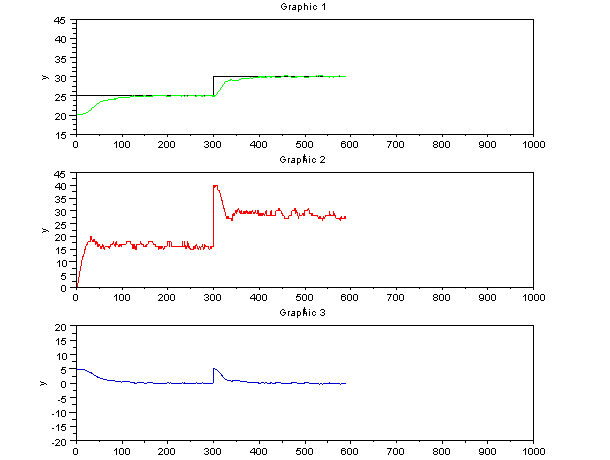
\includegraphics[width=\linewidth]{IMC/imc_092_resp.png}
	\caption{Experimental Results with IMC for $\alpha=0.92$}
	\label{fig:0.991}
\end{figure}[t]
\begin{figure}
	\centering
		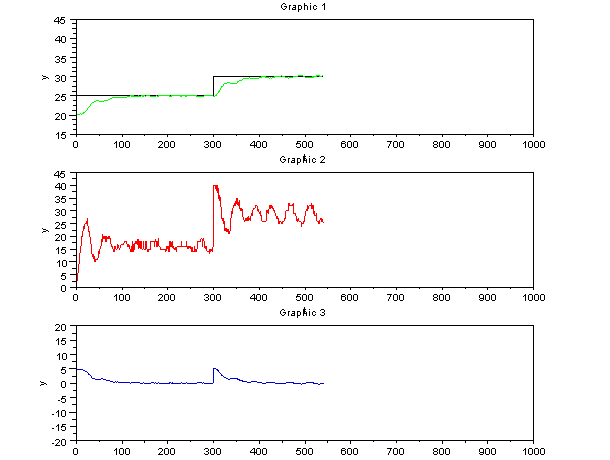
\includegraphics[width=\linewidth]{IMC/imc_085_resp.png}
		\caption{Experimental Results with IMC for $\alpha=0.85$}
	\label{fig:0.98}
\end{figure}
\\By comparing above two graph we can say that for $\alpha=0.92$ the response of the controller is sluggish. For $\alpha=0.85$ the controller starts responding quickly and no overshoots are seen in the temperature profile.


\subsection{Virtually}
The step by step procedure for conducting an experiment virtually is explained in section \ref{vlabsexpt}. The required .sce file is {\tt imc\_virtual.sce}.  You will find this file in the {\tt imc\_controller} directory under {\tt virtual} folder. The necessary codes are listed in the section \ref{imccodes}


\section{Scilab Code}\label{imccodes}
\begin{code}
\ccaption{ser\_init.sce}{\ttfamily ser\_init.sce}
\lstinputlisting{Scilab/local/imc_controller/ser_init.sce}
\end{code}

\begin{code}
 \ccaption{imc.sci}{\ttfamily imc.sci}
\lstinputlisting{Scilab/local/imc_controller/imc.sci}
\end{code}


\begin{code}
 \ccaption{imc\_virtual.sce}{\ttfamily imc\_virtual.sce}
\lstinputlisting{Scilab/virtual/imc_controller/imc_virtual.sce}
\end{code}


\begin{code}
 \ccaption{imc\_virtual.sci}{\ttfamily imc\_virtual.sci}
\lstinputlisting{Scilab/virtual/imc_controller/imc_virtual.sci}
\end{code}


%\bibliography{imc} 
